\documentclass[a4paper,fleqn]{book}

\usepackage{graphicx,amsfonts,psfrag,fancyhdr,layout,appendix,subfigure,amsmath}
\usepackage[sectionbib]{natbib}
\usepackage{chapterbib}

% Set equal margins on book style
\setlength{\oddsidemargin}{53pt}
\setlength{\evensidemargin}{53pt}
\setlength{\marginparwidth}{57pt}
\setlength{\footskip}{30pt}

% Redefine plain page style
\fancypagestyle{plain}{
\fancyhf{}
\renewcommand{\headrulewidth}{0pt}
\fancyfoot[LE,RO]{\thepage}
}

% Code for creating empty pages
% No headers on empty pages before new chapter
\makeatletter
\def\cleardoublepage{\clearpage\if@twoside \ifodd\c@page\else
    \hbox{}
    \thispagestyle{plain}
    \newpage
    \if@twocolumn\hbox{}\newpage\fi\fi\fi}
\makeatother \clearpage{\pagestyle{plain}\cleardoublepage}


% Define pagestyle
\pagestyle{fancy}
\fancyhf{}
\renewcommand{\chaptermark}[1]{\markboth{ \emph{#1}}{}}
\fancyhead[LO]{}
\fancyhead[RE]{\leftmark}
\fancyfoot[LE,RO]{\thepage}

% Dutch style of paragraph formatting, i.e. no indents. 
\setlength{\parskip}{1.3ex plus 0.2ex minus 0.2ex}
\setlength{\parindent}{0pt}

% Less detailed TOC
\setcounter{tocdepth}{2}

\makeindex

% Document starts here
\begin{document}

\frontmatter

\title{A Short Course in Arbitrage Pricing}
\author{Joseph Clark}

\maketitle

%\include preface

% Remove parskip for toc
\setlength{\parskip}{0ex plus 0.5ex minus 0.2ex}
\tableofcontents

% Dutch style of paragraph formatting, i.e. no indents.
\setlength{\parskip}{1.3ex plus 0.2ex minus 0.2ex}

\mainmatter
% Adjustments headers
\fancyhead[LO]{\leftmark}
\fancyhead[RE]{\emph{Chapter \thechapter}}

\chapter{Introduction}
\include{introduction}
\chapter{Fixed income pricing}

\section{The basics}

People who lend money often insist on being paid a rental rate. The rate depends on the period of the loan, the person, the currency, and a number of other factors. Loans are often resold into secondary markets and traded like any other financial asset. The study of money loans is called \textbf{fixed income} (or \textbf{fixed interest}) because the amount of money repaid is generally fixed by agreement, in comparison to other assets where future financial flows are uncertain.

Fixed income is useful to know:  The pricing and analysis of many other products incorporates information about the rental price of money, so it's difficult to understand what's going on with options or futures or more exotic things without knowing a bit about the debt markets.

Three objects will concern us here: \textbf{bonds}, \textbf{zero rates}, \textbf{forward rates}, and \textbf{swap rates}. Understanding these and how to convert between them is fundamental to understanding fixed income markets. We'll start by assuming that all loans are the same except for when they are taken out and repaid.

\subsection{Notation}
Start with some notation. Let $y(t)$ be the interest rate for a loan made now and repaid in $t$ years. The curve for all $t$ is called the \textbf{zero curve} and the component rates \textbf{zero rates}. This is short for `zero coupon', but don't worry about that for now.

Now let $f(t_1,t_2)$ be the interest rate for a loan made at time $t_1$ and paid back at time $t_2$. These are called \textbf{forward rates}.

Unless otherwise noted all rates from here will be continuously compounded. The appendix contains a reminder of how continuous compounding works and how to convert between discrete and continuous compounded rates so $N$ dollars borrowed at rate $y$ for $T$ periods will compound to

\[N\exp (yT) \]


\section{Converting between zero rates and forward rates}


\subsection{General case}

If we have two \textit{zero rates} $y(t_1)$ and $y(t_2)$ we can determine the forward rate $f(t_1,t_2)$ -- the interest rate on a loan taken out at $t_1$ and repaid at $t_2$ -- using an arbitrage argument. The essence of this argument is that it should cost the same to borrow from now to $t_1$, and then at the forward rate from $t_1$ to $t_2$, as it does to simply borrow from now to $t_2$. If this were not true there would be an arbitrage.

In more concrete terms it should cost the same to take out a loan for two years as to take out a loan for one year, and another in a years time at the forward rate (see figure \ref{frArb}) . This gives us the formula for forward rates:

\begin{figure}[htbp]
\begin{center}
  \includegraphics[width=5in]{pics/zt1t2_llb.png} \\
  \caption{Forward rate arbitrage: borrow long, lend short}
\label{frArb}
\end{center}
\end{figure}


\begin{center}
(loan for $t_2$ periods)  = (loan for $t_1$ periods)(loan for $t_2-t_1$ periods)
\[\Rightarrow \exp(y(t_2)t_2) = \exp(y(t_1)t_1)\exp(f(t_1,t_2)(t_2-t_1)) \]
We can solve to get any forward rate:
\begin{equation}f(t_1,t_2) = \frac{y(t_2)t_2-y(t_1)t_1}{t_2-t_1}  \label{fRates}\end{equation}
\end{center}


\subsection{Example} Suppose that $y(1) = 0.05$ and $y(2) = 0.075$. We can see immediately that

\[f(1,2) = \frac{0.075*2-0.05*1}{2-1} = 0.1 \]


Which is to say that the one year rate one year from now (from year one to year two) should be 10\%.

\subsection{Forward rate arbitrage}

If the forward and zero rates does not conform to \ref{fRates} there will be arbitrage. We'll work through a couple of examples to see how this works.

But what if it isn't? What if instead $f(1,2)=0.11$? Then we would have the following arbitrage:
\begin{center}
\begin{tabular}{|c|c|}
  \hline
  % after \\: \hline or \cline{col1-col2} \cline{col3-col4} ...
  time & transaction \\
  \hline
  now & Borrow \$1 for 2 years at 0.075 \\
   & Lend \$1 for 1 year at 0.05 \\
   \hline
  1 & Receive \$ 1$\exp(0.05*1)$ \\
   & Lend \$1$\exp(0.05*1)$ \\
  \hline
  2 & Receive \$1$\exp(0.05*1)\exp(0.11*(2-1))$ \\
   & Repay  \$1 $\exp(0.075*2)$ \\
  \hline
  Profit & \$1$\exp(0.05*1)\exp(0.11*(2-1))-\$1 \exp(0.075*2) = \$0.0117$ \\
  \hline
\end{tabular}
\end{center}

\begin{figure}[htbp]
\begin{center}
  \includegraphics[width=3in]{pics/zt1t2_bbl.png} \\
  \caption{Forward rate arbitrage: borrow short, lend long}
\label{frArb2}
\end{center}
\end{figure}



If instead $f(1,2)=0.09$ we would do the opposite to last time:\\
\begin{center}
\begin{tabular}{|c|c|}
  \hline
  % after \\: \hline or \cline{col1-col2} \cline{col3-col4} ...
  time & transaction \\
  \hline
  now & Lend \$1 for 2 years at 0.075 \\
   & Borrow \$1 for 1 year at 0.05 \\
   \hline
  1 & Repay \$1$\exp(0.05*1)$ \\
   & Borrow \$1$\exp(0.05*1)$ @ 0.11 \\
  \hline
  2 & Repay \$1$\exp(0.05*1)\exp(0.11*(2-1))$ \\
   & Receive  \$1 $\exp(0.075*2)$ \\
  \hline
  Profit & \$1 $\exp(0.075*2)$-\$1$\exp(0.05*1)\exp(0.09*(2-1)) = \$0.0116$ \\
  \hline
\end{tabular}
\end{center}

The general version of the two arbitrages for $y(t_1)$,$y(t_2)$, and $f(t_1,t_2)$ for $0<t_1<t_2$\\

If \[f(t_1,t_2) < \frac{y(t_2)t_2-y(t_1)t_1}{t_2-t_1} \]

then\\
\begin{center}
\begin{tabular}{|c|c|}
  \hline
  % after \\: \hline or \cline{col1-col2} \cline{col3-col4} ...
  time & transaction \\
  \hline
  now & Borrow \$1 for $t_2$ years at $y(t_2)$ \\
   & Lend \$1 for $t_1$ years at $y(t_1)$ \\
   \hline
  1 & Receive \$1$\exp(y(t_1)*t_1)$ \\
   & Lend \$1$\exp(y(t_1)*t_1)$ at $f(t_1,t_2)$ \\
  \hline
  2 & Receive \$1$\exp(y(t_1)*t_1)\exp(f(t_1,t_2)*(t_2-t_1))$ \\
   & Repay  \$1 $\exp(y(t_2)*t_2)$ \\
  \hline
  Profit & \$1$\exp(y(t_1)*t_1)\exp(f(t_1,t_2)*(t_2-t_1))-\$1 \exp(y(t_2)*t_2)>0$  \\
  \hline
\end{tabular}
\end{center}

If \[f(t_1,t_2) > \frac{y(t_2)t_2-y(t_1)t_1}{t_2-t_1} \]

then\\
\begin{center}
\begin{tabular}{|c|c|}
  \hline
  % after \\: \hline or \cline{col1-col2} \cline{col3-col4} ...
  time & transaction \\
  \hline
  now & Lend \$1 for $t_2$ years at $y(t_2)$ \\
   & Borrow \$1 for $t_1$ years at $y(t_1)$ \\
   \hline
  1 & Repay \$1$\exp(y(t_1)*t_1)$ \\
   & Borrow \$1$\exp(y(t_1)*t_1)$ at $f(t_1,t_2)$ \\
  2 & Repay \$1$\exp(y(t_1)*t_1)\exp(f(t_1,t_2)*(t_2-t_1))$ \\
   & Receive  \$1 $\exp(y(t_2)*t_2)$ \\
  \hline
  Profit & $\$1 \exp(y(t_2)*t_2)-\$1 \exp(y(t_1)*t_1)\exp(f(t_1,t_2)*(t_2-t_1))>0$  \\
  \hline
\end{tabular}
\end{center}

This should be enough to convince us that the relationship in \ref{fRates} holds nearly exactly. Forward rate arbitrage, when it exists, will be gobbled up very quickly amongst the deep liquidity and tight spreads of the bond markets.

\section{Determining zero rates from bond prices}

Life would be easier if all bonds were simple borrow-at-$t_1$-repay-at-$t_2$ type arrangements. If they were the relationship between the price and yield of of a bond would be

\begin{eqnarray*}
P(0) &=& F\exp (-y(t)t)\\ \mbox{ or, in terms of yield, }\\
y(t) &=& -\ln \left( \frac{P(0)}{F} \right)1/t
\end{eqnarray*}

So a bond that paid \$100 in 5 years time which currently traded at \$67 could be revealed to have a yield of

\[0.0801 = -\ln \left( \frac{67}{100} \right)1/5\]

But life wasn't meant to be easy, and bonds have a nasty habit of paying a regular sequence of payments (called \textbf{coupons}) and then a final payment (called the \textbf{face value}). This complicates things a bit.

\subsection{Determining the price of a bond with coupons}

\subsubsection{Example}
We might have a 5 year bond with a 6\% coupon and \$100 face value that pays a \$6 coupon every year and \$100 after 5 years. What's the yield and price of this bond?

This bond is really easy to price. We just note that any payment $FV$ that occurs in the future in $t$ years is worth \[PV = F\exp(-y(t)t)  \]
where $y(t)$ is the interest rate

The payments [6,6,6,6,6+100] at times [1,2,3,4,5] are therefore worth
\begin{eqnarray*}P = 6\exp(-y(1)*1)+6\exp(-y(2)*2)\\+6\exp(-y(3)*3)+6\exp(-y(4)*4)\\+(6+100)\exp(-y(5)*5)\end{eqnarray*}

\subsubsection{General case}
In general for a stream of coupons $[C_1,...,C_N]$ at times $[t_1,\ldots,t_N]$ with and a face value of $F$ with rates of

\begin{equation}P = \left[\sum_{j=1}^N C_j\exp(-y(t_j)t_j)\right] + F \exp(-y(t_N)t_N)  \label{bondPrice}\end{equation}

This is the bond pricing formula.

\subsection{Determining the yield of a bond with coupons}

\subsubsection{General case}
The \textit{yield} of a bond is the unique interest rate that satisfies the price. Just drop the argument from the interest rates and solve!

\begin{eqnarray*}
P = \left[\sum_{j=1}^N C_j\exp(-yt_j)\right] + F \exp(-yt_N) \\
y = \ldots
\end{eqnarray*}
It's a bit tricky to solve directly but you get the idea. In practice these problems are solved by choosing a value of $y$ that makes $P- \left[\sum_{j=1}^N C_j\exp(-yt_j)\right] - F \exp(-yt_N)$ as close as possible to zero. This can easily done easily with a spreadsheet or mathematical package.

\subsection{Generating the zero curve from coupon bond prices}

Now the useful part: We will typically have prices for a number of coupon bonds, from which the coupon yields can be fairly easily calculated. It is a bit more difficult to extract the zero rates $y(t)$ from these prices. To do this we use an iterative process called \textbf{bootstrapping}.

Start by noting that all the repayments from a bond, coupons and face value, can be considered in isolation as zero coupon bonds. If we are able to determine the shortest (to maturity) zero rate, we can use it to obtain the next shortest rate, and so on.

\subsubsection{Example} Suppose we have three bonds: a 1/2 year, a 1 year, and a 1.5 year. Each bond pays semi-annual coupons and the face value at maturity. We know the price of each bond, as well as the coupons and face values, and we want to find the zero-coupon rates. The prices are in the table below

\begin{tabular}{|c|c|c|c|c|}
  \hline
  % after \\: \hline or \cline{col1-col2} \cline{col3-col4} ...
  maturity & coupon rate & coupon frequency & face value ($F$) & price ($P$) \\
  \hline
  $t_1 = 0.5$ & 10\%  & semi-annual & 100 & 99 \\
  $t_2 = 1$ & 10\%  & semi-annual & 100 & 96 \\
  $t_3 = 1.5$ & 10\% & semi-annual & 100 & 95 \\
  \hline
\end{tabular}

We can quickly discover the first zero rate $y(0)$ by using the bond pricing formula \ref{bondPrice}. We have

\begin{eqnarray*}
P = \left[\sum_{j=1}^N C_j\exp(-y(t_j)t_j)\right] + F \exp(-y(t_N)t_N) \\
\Rightarrow P(0.5) = \left[C_1\exp(-y(0.5)0.5)\right] + F \exp(-y(0.5)0.5) \\
\Rightarrow y(0.5) &=& \frac{1}{t_1}\ln\left(\frac{F+C}{P(0.5)}\right) \\
&=& \frac{1}{0.5}\ln\left(\frac{100+5}{99}\right) = 0.1177 \\
\end{eqnarray*}

So the zero coupon rate for maturity of 1/2 a year is 11.77\% Splendid.

 Now we can use this to obtain the 1 year zero coupon rate. We again start with the bond pricing formula and substitute in for the one year bond, using our result for $y(0.5)$ from the last step.

\begin{eqnarray*}
P = \left[\sum_{j=1}^N C_j\exp(-y(t_j)t_j)\right] + F \exp(-y(t_N)t_N)\\
\Rightarrow P(1) = \frac{C_1}{\exp(y(0.5)*0.5)} +\frac{F+C_2}{\exp(y(1)*1)}\\
\Rightarrow y(1) &=& \ln \left(\frac{F+C_2}{P(1)-\frac{C_1}{\exp(y(0.5)*0.5)}} \right)\\
 &=& \ln \left(\frac{100+5}{96-\frac{5}{\exp(0.1177*0.5)}} \right) = 0.14
\end{eqnarray*}

Things are going well. Now we have the 1/2 year rate and the 1 year zero rate. Note that this is different from the yields on those two bonds. The zero rates are more informative, which is why we are willing to spend all this trouble obtaining them.

The third step is the same again:

\begin{eqnarray*}
P = \left[\sum_{j=1}^N C_j\exp(-y(t_j)t_j)\right] + F \exp(-y(t_N)t_N)\\
P(1.5) = \frac{C_1}{\exp(y(0.5)*0.5)} +\frac{C_2}{\exp(y(1)*1)}+\frac{F+C_3}{\exp(y(1)*1)}\\
\Rightarrow y(1.5) = 0.1335
\end{eqnarray*}

Now we have all the zero rates. This schedule of rates $y(0.5) = 0.1177$, $y(1)=0.14$, $y(1.5) = 0.1335$ is called the \textbf{zero coupon curve} and represents the continuously compounded interest rates for a simple loans with these maturities.

\subsubsection{General case}
In general for a stream of coupons $[C_1,...,C_N]$ at times $[t_1,\ldots,t_N]$ with and a face value of $F$ the $N$'th zero coupon yield is given by

\begin{equation}
y(t_N) = \frac{1}{t_N} \ln \left( \frac{C_N +F}{P(t_N)-\sum_{i=1}^{N-1}\exp(-C_{j}y(t_j)t_j))} \right)
\end{equation}

\subsubsection{Arbitrage}

If zero rates differ from our calculated zero curve we can construct an arbitrage. To keep things simple lets assume that the bonds in the table are offered and there are also a yield curve $y(0.5)=y(1)=y(1.5)=0.1$. Say we want to arbitrage the 1.5 year bond, we construct the arbitrage by buying the bond financed by a 1.5 year loan at 10\%. We'll get paid three coupons of \$5 each. The first two we'll reinvest at the forward rates $f(0.5,1.5)$ and $f(1,1.5)$. The last one will be paid at maturity along with the face value of \$100.

The forward rates are 

\begin{eqnarray*}
f(t_1,t_2) &=& \frac{y(t_2)t_2-y(t_1)t_1}{t_2-t_1}\\
\Rightarrow f(0.5,1.5) &=& \frac{y(1.5)1.5-y(0.5)0.5}{1.5-0.5}\\
&=& \frac{0.1*1.5-0.1*0.5}{1.5-0.5}\\
&=& 0.1\\
            f(1,1.5) &=& \frac{y(1.5)1.5-y(1)1}{1.5-1}\\
            &=& \frac{0.1*1.5-0.1*1}{1.5-1}\\
            &=& 0.1
\end{eqnarray*}


The arbitrage looks like this

\begin{center}
\begin{tabular}{|c|c|}
  \hline
  % after \\: \hline or \cline{col1-col2} \cline{col3-col4} ...
  time & transaction \\
  \hline
  now & Borrow \$95 for 1.5 years at 0.1 \\
   & Buy 1.5 year bond \\
   \hline
  0.5 & Receive \$5 coupon \\
   & Invest \$5 coupon at f(0.5,1.5)\\
  \hline
  1 & Receive \$5 coupon \\
   & Invest \$5 coupon at f(1,1.5)\\
  \hline
  1.5 & Receive \$5 coupon \\
      & Receive first reinvested coupon: $5\exp (0.1*1)=5.5259$\\
      & Receive first reinvested coupon: $5\exp (0.1*0.5)=5.2564$\\
      & Receive \$100 face value\\
      & Repay loan: $95\exp (0.1*1.5) = 110.37$\\
  \hline
  Profit & 5.5259+5.2564+100-110.37 = 0.4122 \\
  \hline
\end{tabular}
\end{center}

\textbf{Exercise:} Construct an arbitrage if the yield curve were $y(0.5)=y(1)=y(1.5)=0.15$

\section{Converting forward rates to swap rates}

A swap is a financial contract to swap a series of payments over time. There are three types of swaps
\begin{enumerate}
\item \textit{Fixed-Fixed}: One fixed payment against another. e.g. pay 1 apple per week for 10 weeks, receive 1 banana per week for 10 weeks.
\item \textit{Fixed-Floating:} One side is fixed and the other side is determined by something that hasn't happened yet. e.g. pay 6\% times \$100 per year for 10 years against the Fed funds rate times \$100 per year for 10 years.
\item \textit{Floating-Floating:} Both sides are floating. e.g. pay RBA cash rate times \$100 per year for 10 years, receive 2\%+ Fed funds rate per year for 10 years.
\end{enumerate}

In the simplest type of swap the floating side of the swap is paid \textit{after} the rate is set. So, for instance, if the agreement is to pay 90 day BBSW, the exchange occurs 90 days after the as yet unknown BBSW is observed. The payment date is sometimes called the \textbf{anniversary date}. 

There are other types of swaps where payments are exchanged on the date that the floating rate is observed. These are called \textbf{in arrears swaps} but they're a bit tricky to price so we won't cover them here.

We'll need a slight change in notation to talk about future spot rates. We'll call $y(t,T)$ the zero rate observed at time $t$ for a loan starting at $t$ and maturing at $T$. In the previous sections we have been talking about rates observed now so $y(1) \equiv y(0,1)$ etc.

An additional irritation is that we will be using both simple (period by period) and continuously compounded rates for reasons that become clear when you look at the hedging arguments. We'll use the subscript $s$ to denote the simple rate. If you lend \$1 at the simple rate $y_s(0,T)$ for $T$ periods you get $\$1(1+y_s(0,T))^T$ back when the loan is due. Simple rates have a straightforward relationship to continuously compounded rates:

\[ y_s(t,T) = e^{y(t,T)}-1\]

\subsection{The big idea}

A swap is a series of known and unknown payments. To price a swap correctly we find instruments to hedge out all the unknown payments. We generally do this with forwards. Once we remove the uncertain elements we can quickly determine the swap rate that gives a present value of zero. Any deviation from this gives us an arbitrage.

Say we agree now at time $t=0$ to borrow \$1 at the forward rate $f(1,2)$ in one year's time. At $t=1$ we can borrow at the agreed rate and lend at the prevailing rate $y(1,2)$. At $t=2$ we repay the forward-price loan for $\$1e^{f(1,2)}$ and receive payment on the other loan for $\$1e^{y(1,2)}$. The payoff is

\[ \$1e^{f(1,2)} -\$1e^{y(1,2)} \]

This trade has a negative exposure to $y(1,2)$. We can use trades like this to offset unwanted exposures to the rate. We can do the trade in reverse to generate the positive exposure. This is the trick we will use to value the floating parts of swaps. 

\subsection{Swap-forward arbitrage}

We'll explore the arbitrage argument with generic one and two period swaps.\\

\textbf{Example: a one period swap}\\

The best place to start is with only one exchange of payments. In this example we agree at $t=0$ to exchange $\$1*y_s(1,2)$ for some swap rate $\$1*SW$ at $t=2$. Note that we pay the $y_s(1,2)$ on the anniversary ($t=2$) one year after we observe it. What should $SW$ be? 

\begin{figure}[htbp]
\begin{center}
  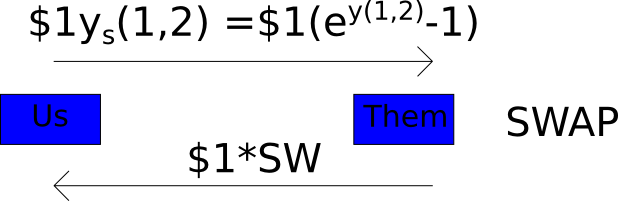
\includegraphics[width=3in]{pics/swap1P.png} \\
  \caption{Swap at t=2}
\label{swap1P}
\end{center}
\end{figure}

The answer comes from an arbitrage argument. We will hedge the floating payment with forwards and then find the swap rate that makes the combined value of all fixed and floating payments equal to zero. If they are not zero we have an arbitrage.

Say we recieve the fixed rate and pay the floating rate. The most obvious (and correct) hedge is a forward contract to borrow \$1 from $t=1$ to $t=2$. This rate is $f(1,2)$. At $t=1$ we lend out this \$1 for a year at the prevailing rate $y(1,2)$.

The table below gives the story of the swap and the hedge:

\begin{tiny}
\begin{tabular}{|c|c|c|}
\hline
time & contract/action & cashflow\\
\hline
0 & \begin{tabular}{c}Enter swap to pay $\$1*y_s(1,2)$ and receive $\$1*SW$\\ Enter forward to borrow \$1 at $f(1,2)$\\ \end{tabular} & 0\\
\hline
1 & \begin{tabular}{c}Borrow \$1 at $f(1,2)$\\ Lend \$1 at $y(1,2)$ \end{tabular} & 0\\
\hline
2 & & \begin{tabular}{c}Pay $\$1e^{f(1,2)}$ from loan\\ Receive $\$1e^{(y(1,2)}$ from loan\\ Pay $\$1y_s(1,2)$ from swap \\ Receive $\$1SW$ from swap\\  \end{tabular}\\
\hline
\end{tabular}
\end{tiny}

We can divide the cashflows into those coming from loans (including the loan at the forward rate) and the fixed and floating side of the swap. We'll also discount everything at $t=2$ by $y(0,2)$:

\begin{tiny}
\begin{tabular}{|c|c|c|c|}
\hline
time & value of loans & value of floating & value of fixed\\
\hline
0 & 0 & 0 & 0\\ 
1 & 0 & 0 & 0\\
2 & $e^{-y(0,2)}(\$1e^{y(1,2)}-\$1e^{f{1,2}})$ & $-e^{-y(0,2)}(\$1*y_s(1,2) = -e^{-y(0,2)}(\$1*(e^{y(1,2)}-1))$ & $e^{-y(0,2)}*\$1*SW$\\
\hline
\end{tabular}
\end{tiny}

Note that we substitute out $y_s$ with $y_s = e^y-1$. From here the swap rate $SW$ is easy to find. Since the portfolio is self financed it should give zero profit. The no-arbitrage condition is:

\begin{eqnarray*}
e^{-y(0,2)}(\$1e^{y(1,2)}-\$1e^{f{1,2}})-e^{-y(0,2)}(\$1*(e^{y(1,2)}-1))+e^{-y(0,2)}*\$1*SW = 0\\
\Rightarrow SW = e^{f(1,2)-1}
\end{eqnarray*}

The forward has done its job and offset the exposure to the floating rate. Figure \ref{swapAndHedge} tells the story:

\begin{figure}[htbp]
\begin{center}
  \includegraphics[width=3in]{pics/swapAndHedge.png} \\
  \caption{Swap and hedge combined at at $t=2$}
\label{swapAndHedge}
\end{center}
\end{figure}


\textbf{Example: Two period swap}\\

A two period swap adds one extra exchange: in period $t=3$ we exchange $\$1*y_s(2,3)$ for the swap rate $\$1*SW$ 

\begin{figure}[htbp]
\begin{center}
  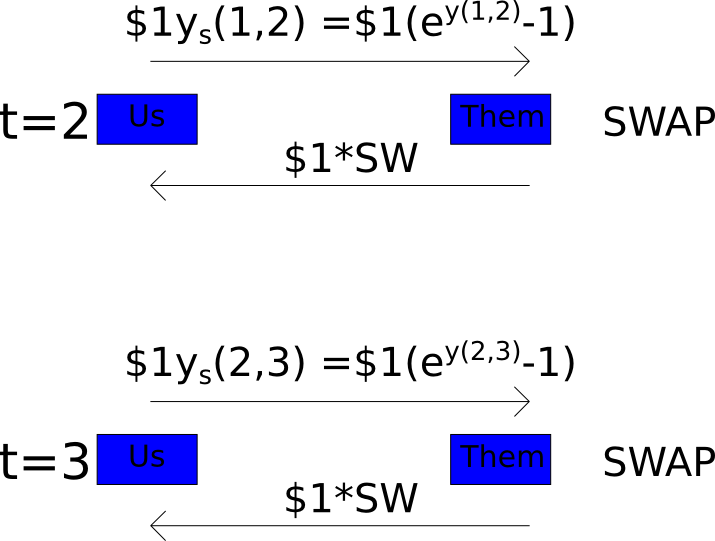
\includegraphics[width=3in]{pics/swap2P.png} \\
  \caption{Swap at $t=2$ and $t=3$}
\label{swap2P}
\end{center}
\end{figure}

Now we have to worry about two floating rates: $y_s(1,2)$ and $y_s(2,3)$. Since we pay the floating rate we need to borrow at the forward rate in $t=1$ and $t=2$ to offset. 

\begin{tiny}
\begin{tabular}{|c|c|c|}
\hline
time & contract/action & cashflow\\
\hline
0 & \begin{tabular}{c}Enter swap to pay $\$1*y_s(t-1,t)$ and receive $\$1*SW$ at $t=2,3$\\ Enter forwards to borrow \$1 at $f(t-1,t)$ for $t=2,3$\\ \end{tabular} & 0\\
\hline
1 & \begin{tabular}{c}Borrow \$1 at $f(1,2)$\\ Lend \$1 at $y(1,2)$ \end{tabular} & 0\\
\hline
2 &\begin{tabular}{c}\\ Borrow \$1 at $f(2,3)$\\ Lend \$1 at $y(2,3)$  \end{tabular}  & \begin{tabular}{c}Pay $\$1\exp(f(1,2))$ from loan\\ Receive $\$1\exp(y(1,2))$ from loan\\ Pay $\$1y_s(1,2)$ on swap \\ Receive $\$1SW$ from swap\\ \end{tabular}\\
\hline
3 & & \begin{tabular}{c}Pay $\$1\exp(f(2,3))$ from loan\\ Receive $\$1\exp(y(2,3))$ from loan\\ Pay $\$1y_s(2,3)$ on swap \\ Receive $\$1SW$ from swap\\ \end{tabular}\\
\hline
\end{tabular}\\
\end{tiny}

The discounted values of all the cashflows are summarised here 

\begin{tiny}
\begin{tabular}{|c|c|c|c|}
\hline
time & value of loans & value of floating & value of fixed\\
\hline
0 & 0 & 0 & 0\\ 
1 & 0 & 0 & 0\\
2 & $e^{-y(0,2)}(\$1e^{y(1,2)}-\$1e^{f(1,2)})$ & $-e^{-y(0,2)}\$1*y_s(1,2) = -e^{-y(0,2)}(\$1*(e^{y(1,2)}-1))$ & $e^{-y(0,2)}*\$1*SW$\\
3 & $e^{-y(0,3)}(\$1e^{y(2,3)}-\$1e^{f(2,3)})$ & $-e^{-y(0,3)}\$1*y_s(2,3) = -e^{-y(0,3)}(\$1*(e^{y(2,3)}-1))$ & $e^{-y(0,3)}*\$1*SW$\\
\hline
\end{tabular}
\end{tiny}

Since these are all in $t=0$ values we can sum up and set equal to zero to find the swap rate:

\[SW | \sum_{\tau=2}^3  e^{-y(0,\tau)}(1-e^{f(\tau-1,\tau)} +SW) = 0 \]

It's a simple matter to find $SW$ that satisfies this equation.

\subsection{The general formula}

The previous example easily generalises to an arbitrary number of periods. For a swap fixing at $t, t+1 \ldots T$ with anniversaries at $t+1,t+2,\ldots,T+1$ the swap price satisfies

\begin{eqnarray}
SW  | \sum_{\tau=t+1}^{T+1}  e^{-y(0,\tau)\tau}(e^{f(\tau-1,\tau)}-1 -SW) = 0  \label{swapprice}
\end{eqnarray}

Notice that since all cashflows are multiples of the notional value we can divide them out  without changing the result. 

This is an intuitive formula. It says \textbf{the sum of discounted differences between the (simple) forward rate and the swap rate should be zero}.

Some swaps pay fixed and floating rates at different times. It's easy to accommodate these. Let $N_F(t)$ and $N_L(t)$ be the fixed and floating notional values. Then 

\begin{eqnarray*}
SW  | \sum_{\tau=t+1}^{T+1}  e^{-y(0,\tau)\tau}N_L(t)(e^{f(\tau-1,\tau)}-1)  - e^{-y(0,\tau)\tau}N_F(t)SW = 0  \label{swapgeneral}
\end{eqnarray*}

We just have to remember to borrow $N_L(t)$ to construct the hedge. With swaps with asyncronous payments sometimes $N_L(t)$ and $N_F(t)$ will be zero. Our formula works fine with this.


\subsection{Worked example: 3 period swap}

\textit{Step 1: Calculate forward rates}\\

Suppose we have the following zero rates:\\
\begin{center}
\begin{tabular}{|c|c|}
  \hline
  % after \\: \hline or \cline{col1-col2} \cline{col3-col4} ...
  $t$ & $y(0,t)$ \\
  \hline
  1&0.05 \\
  2&0.06 \\
  3&0.09 \\
  4&0.08 \\
  5&0.07\\
  \hline
\end{tabular}
\end{center}
We can calculate the forward rates\\
\begin{center}
\begin{tabular}{|c|c|c|}
  \hline
  % after \\: \hline or \cline{col1-col2} \cline{col3-col4} ...
  $t$ & $y(0,t)$ & $f(t,t+1)$ \\
  \hline
  1&0.05 & 0.07\\
  2&0.06 & 0.15\\
  3&0.09 & 0.05 \\
  4&0.08 & 0.03\\
  \hline
\end{tabular}
\end{center}

\textit{Step 2: Construct discounted payoff and solve for swap rate}\\

We can use the general formula

\begin{eqnarray*}
\sum_{\tau=t+1}^{T+1}  e^{-y(0,\tau)}(e^{f(\tau-1,\tau)}-1 -SW) = 0 \\
\Rightarrow e^{-y(0,2)2}(e^{f(1,2)} - 1 - SW) + e^{-y(0,3)3}(e^{f(2,3)} - 1 - SW)+ e^{-y(0,4)4}(e^{f(3,4)} - 1 - SW) =0\\
\Rightarrow e^{-0.06*2}(e^{0.07} - 1 - SW) + e^{-0.09*3}(e^{0.015} - 1 - SW)+ e^{-0.08*4}(e^{0.05} - 1 - SW) =0\\
\Rightarrow SW = 0.094\\
\end{eqnarray*}

So the swap rate is 0.094.

\section{Questions}

\textbf{Question 1:}\\
Calculate the price for a bond that pays a coupon of \$10 per year for 5 years with a \$50 face value if the zero curve is constant at 3\%.

\textbf{Question 2:}\\
If the one year interest rate is $y(1) = 0.02$ and the 5 year interest rate is $y(5) = 0.03$ calculate the 4 year interest rate 1 year forward.

\textbf{Question 3:}\\
Suppose we have the following zero rates:\\
\begin{center}
\begin{tabular}{|c|c|}
  \hline
  % after \\: \hline or \cline{col1-col2} \cline{col3-col4} ...
  $t$ & $y(t)$ \\
  \hline
  1&0.05 \\
  2&0.06 \\
  3&0.07 \\
  4&0.08 \\
  5&0.09\\
  \hline
\end{tabular}
\end{center}


Consider a swap to receive \$1,000,000 times a some fixed swap rate $SW$ each year and pay \$1,000,000 times the one year zero rate $y(t-1,t)$ for four years starting at $t=2$. Calculate the no-arbitrage value of $SW$. (hint: you'll need to use a spreadsheet or mathematical package)



\section*{Appendix: Compounding}


So let's say I borrow \$1 and repay the loan in $t$ years from now with an annual rate of interest $ARI$ paid at the end of each year. I will repay

\[ \$1\underbrace{\left(1+\mbox{ARI}\right)\left(1+\mbox{ARI}\right)\ldots\left(1+\mbox{ARI}\right)}_{\mbox{t times}} \]


or

 \[\$1\left(1+\mbox{ARI}\right)^t \]

Suppose instead that the interest is paid semi-annually. I will now repay \[\$1\left(1+\frac{\mbox{ARI}}{2}\right)^{2t} \]

Suppose instead that the interest is paid quarterly. I will now repay \[\$1\left(1+\frac{\mbox{ARI}}{4}\right)^{4t} \]

Suppose I pay the interest every day. I will now repay \[\$1\left(1+\frac{\mbox{ARI}}{365}\right)^{365t} \]

As the frequency of repayment approaches infinity the repayments will approach \[\lim_{k\rightarrow\infty}\$1\left(1+\frac{\mbox{ARI}}{k}\right)^{kt} = \$1\exp(rt) \]

where $r$ is the \textit{continuously compounded interest rate}.

Say I borrow \$1 with $ARI = 1$ (100\% per year)

\begin{center}
\begin{tabular}{|p{8cm}|p{8cm}|}
  \hline
  % after \\: \hline or \cline{col1-col2} \cline{col3-col4} ...
  k (frequency of repayments) & repayments (one year)  \\
  \hline
  1 & $\$1\left(1+\frac{1}{1}\right)^{1*1} = \$2 $ \\
  4 & $\$1\left(1+\frac{1}{4}\right)^{4*1} = \$2.441406$ \\
  365 & $\$1\left(1+\frac{1}{365}\right)^{365*1} = \$2.714567$\\
  1000 & $\$1\left(1+\frac{1}{1000}\right)^{1000*1*} = \$2.716924 $  \\
  $\infty$ & $\lim_{k\rightarrow\infty}\$1\left(1+\frac{1}{k}\right)^{k*1} = \exp(1*1) \approx \$2.718282$\\
  \hline
\end{tabular}
\end{center}

The number 2.71828182845709... is called $e$. The expression $e^x$ is often written as $\exp(x)$. It is a very important number. If a variable $x$ grows at a rate $g$ for $t$ periods of compounded growth starting at $x(0)$ then its value at time $t$ will be

\[x(t) = x(0)\exp(gt) \]

Back to borrowing. Say I borrow \$1 with $ARI = 0.05$ (5\% per year) for one year
\begin{center}
\begin{tabular}{|p{8cm}|p{8cm}|}
  \hline
  % after \\: \hline or \cline{col1-col2} \cline{col3-col4} ...
  k (frequency of repayments) & repayments (one year) \\
  \hline
  1 & $\$1(1+\frac{0.05}{1})^{1*1} = \$1.05 $  \\
  4 & $\$1(1+\frac{0.05}{4})^{4*1} = \$1.050945$ \\
  365 & $\$1(1+\frac{0.05}{365})^{365*1} = \$1.0512675$ \\
  1000 & $\$1(1+\frac{0.05}{1000})^{1000*1} = \$1.051270 $ \\
  $\infty$ & $\lim_{k\rightarrow\infty}\$1(1+\frac{0.05}{k})^{k*1} = \exp(0.05*1) \approx \$1.051271$\\
  \hline
\end{tabular}
\end{center}

Say I borrow \$1 with $ARI = 0.05$ (5\% per year) for two years
\begin{center}
\begin{tabular}{|p{8cm}|p{8cm}|}
  \hline
  % after \\: \hline or \cline{col1-col2} \cline{col3-col4} ...
  k (frequency of repayments) & repayments (two years) \\
  \hline
  1 & $\$1(1+\frac{0.05}{1})^{1*2} = \$1.1025 $ \\
  4 & $\$1(1+\frac{0.05}{4})^{4*2} = \$1.104486$\\
  365 & $\$1(1+\frac{0.05}{365})^{365*2} = \$1.105163$ \\
  1000 &  $\$1(1+\frac{0.05}{1000})^{1000*2*} = \$1.105168 $  \\
  $\infty$ & $\lim_{k\rightarrow\infty}\$1(1+\frac{0.05}{k})^{k*2} = \exp(0.05*2) \approx \$1.105171$ \\
  \hline
\end{tabular}
\end{center}


We can convert between the $ARI$ and $y$ by comparing a discretely compounded loan with a continuously compounded loan
\begin{eqnarray*}
\mbox{discrete} & =\mbox{continuous}\\
\rightarrow \$1\left(1+\frac{\mbox{ARI}}{k}\right)^{kt} & = \exp(yt)
\end{eqnarray*}
\begin{equation}
\rightarrow y = k \ln \left(1+\frac{\mbox{ARI}}{k} \right)
\end{equation}


So in summary we have:

\textit{Discrete compounding:}

\[FV_{\mbox{discrete}} = \mbox{PV}\left(1+\frac{ARI}{k}\right)^{kt} \]

\textit{Continuous compounding:}

\[FV_{\mbox{continuous}} = \mbox{PV}\exp(yt) \]

We can also use this to discount payoffs which occur in the future by:

\[FV\exp(-yt) = \mbox{PV} \]


\textit{Converting between discrete and continuous compounding:}

\[FV_{\mbox{continuous}} = FV_{\mbox{discrete}} \rightarrow y = k \ln \left(1+\frac{ARI}{k} \right)\]

where
\begin{itemize}
\item PV: present value of loan\\
\item FV: future value of loan\\
\item ARI: annual rate of interest (discrete)\\
\item $k$: number of compounding periods per year\\
\item $t$: number of years\\
\item $y$: continuously compounded interest rate
\end{itemize}






\chapter{Futures pricing}

\section{The basics}

If I wish to purchase a share of a company in one year's time how much should I pay? 

The most obvious answer is that the price should reflect my expectations of the value of the company in one year, possibly adjusted for risk and discounting. This answer is wrong. In most cases the price of such a contract is fixed by arbitrage. Expectations of future value play absolutely no role in pricing such forward contracts. Nor does the riskiness of the price. Or any other considerations except the current price, the interest rate, and any financial flows (such as dividends or coupons) attached to a security.

Except for commodities, which are a little strange. 

Here we will outline the basic logic behind futures arbitrage and sketch the pricing for equities (with and without dividends), currencies, and commodities. 

\subsection{Notation}
Let the price of a security at time $0$ be $S(0)$. The price of a contract to buy or sell $S$ at a future time $T$ is $F_T(0)$. To \textbf{buy}/\textbf{sell} the future is to be obliged to buy/sell the security at $T$. Set the interest rate for a $T$ period loan at $r$. This is a \textbf{zero} rate. For simplicity we can set the zero curve at $r$ for all maturities. 

\section{What's a repo?}
To construct the arbitrage arguments we allow \textbf{short selling}. Short selling creates the opposite cash-flow as a normal purchase. Short sales are created through a transaction called a \textbf{repurchase agreement} or \textbf{repo}. 

A repo for a security $S$ involves borrowing some amount of the security and then repaying the same amount at some future time. Say we borrow at time 0 and immediately sell the security for $S(0)$ which we invest at rate $r$. We then re-acquire the security at time $T$ for $S(T)$ and repay the loan. The cash-flow generated by this transaction is $S(0)(1+r)^T-S(T)$. The opposite transaction is to borrow $S(0)$ to buy the security and then sell it at $T$ for $S(T)$. The cash-flow from this opposite transaction is $S(T) -S(0)(1+r)^T$. Figure \ref{ccrcc} illustrates. 

This is a very useful process as it gives us the mirror image payoff. This is  a useful property for arbitrage. 

\textbf{Remark: (what is the repo rate?)} Above we have assumed that someone is willing to lend the security for $T$ periods and receive no rental rate. This is somewhat unrealistic. But not too unrealistic. Provided that the security doesn't generate any payments (like dividends) the renter is not disadvantaged by the transaction: he is in precisely the same financial situation if he rents or not. He should therefore be indifferent between renting and not renting and so only require a small compensation (a small rate $\epsilon$, or, if you like, a cheap brass trinket). Of course he would prefer more but competitive pressures force him to accept the trinket or settle for nothing.

Owners of securities are regularly paid non-trivial rental rates (\textbf{repo rates}). There are various reasons for this: there is a credit risk associated with the loan (though this can be reduced to a trivial level by margining the loan). If a stock pays dividends the lender will need to be compensated for the loss, but as we will see this and other flows like bond coupons can easily be incorporated into the futures price. There's another big reason, possibly the main reason, but we'll get to that later.

\section{Arbitrage pricing with futures}
 
Futures are priced by constructing arbitrage portfolios that hedge the exposure from the long or short future. The arbitrage process for a short future is called \textbf{cash and carry}; for a long future it is called \textbf{reverse cash and carry}. 

\begin{itemize}
\item \textbf{The cash and carry portfolio}: Buy the security with borrowed money and hold. Sell the futures contract. 
\item \textbf{The reverse cash and carry portfolio}: Repo the security, sell at market, and invest at the risk free rate. Buy the futures contract.
\end{itemize}


%model
%\begin{tiny}
%\begin{tabular}{cc|c|c}
%&$\rightarrow$ & Deliver stock for $F_T(0)$ & T\\ 
% & & Repay loan: $S(0)(+r)^T$ & \\
%\hline
%\textsc{Cash and carry}&$\uparrow$ & & Receive stock for $F_T(0)$\\
%& Sell future @ $F_{T}(0)$    & &   Receive proceeds of loan: $S(0)(1+r)^T$ \\
%& Borrow cash $S(0)$ @ $r$ & & Repay repo \\
%& Buy stock @ $S(0)$ (hold)  & & \\
%\hline
%& 0  & Buy future @ $F_{T}(0)$ $\rightarrow$ & $\uparrow$ \\
%& &  Borrow stock & \\
%&& Sell stock @ $S(0)$ & \\
%&  & Invest $S(0)$ @ $r$ & \\
%& & \textsc{Reverse cash and carry} & \\
%\end{tabular}
%\end{tiny}


\begin{tiny}
\begin{table}
\begin{tabular}{cc|c|c}
&$\rightarrow$ & Deliver stock & T\\ 
 & & Repay loan & \\
\hline
\textsc{Cash and carry}&$\uparrow$ & & Receive stock\\
& Sell future    & &   Receive proceeds of loan \\
& Borrow cash & & Repay repo \\
& Buy stock (hold)  & & \\
\hline
& 0  & Buy future  $\rightarrow$ & $\uparrow$ \\
& &  Borrow stock & \\
&& Sell stock  & \\
&  & Invest cash & \\
& & \textsc{Reverse cash and carry} & \\
\end{tabular}\label{ccrcc}
\caption{Cash and carry and reverse cash and carry}
\end{table}
\end{tiny}


We'll consider four cases: equities with and without dividends, currencies, and commodities. These are arranged from least to most complicated. We'll use discrete compounding to make the analysis simple. The continuously compounded results are straightforward extensions.

\subsection{Equity futures}


\subsubsection{General case}

\textit{Cash and carry:}

\begin{center} \begin{tabular}{|c|c|}
  \hline
  % after \\: \hline or \cline{col1-col2} \cline{col3-col4} ...
  time & action \\
  \hline
  t & Sell future @ $F_{T}(0)$  \\
    & Borrow cash $S(0)$ @ $r$ \\
    & Buy stock @ $S(0)$ (hold) \\
  \hline
 T & Deliver stock for $F_T(0)$ \\
   & Repay loan: $S(0)(+r)^T$ \\
  \hline
   & $F_{T}(0) - S(0)(1+r)^{T}$\\
  \hline
\end{tabular}\end{center}

\textit{Reverse cash and carry:}

\begin{center} \begin{tabular}{|c|c|}
  \hline
  % after \\: \hline or \cline{col1-col2} \cline{col3-col4} ...
  time & action \\
  \hline
  t & Buy future @ $F_{T}(0)$  \\
    & Borrow stock \\
    & Sell stock @ $S(0)$  \\
    & Invest $S(0)$ @ $r$\\
  \hline
  T & Receive stock for $F_T(0)$ \\
    & Receive proceeds of loan: $S(0)(1+r)^T$\\
    & Repay repo \\
  \hline
   & $S(0)(1+r)^{T}-F_{T}(0)$\\
  \hline
\end{tabular}\end{center}

Both these transactions cannot be profitable for there to be no arbitrage. This requires

\[S(0)(1+r)^{T}-F_{T}(0) \leq 0 \]
and
\[F_{T}(0)-S(0)(1+r)^{T} \leq 0 \]
which implies
\[ F_{T}(0) = S(0)(1+r)^{T}  \]

\subsubsection{Example}

\textbf{Non dividend paying stock}

Current price: $S(0)$ = \$100\\
Borrowing/lending: $r$ = 0.05\\
Futures expiry: 1 year\\
Futures price: 100(1+0.05) = \$105 

\subsubsection{Arbitrage}


Say future is 110:

\begin{center} \begin{tabular}{|c|c|}
  \hline
  % after \\: \hline or \cline{col1-col2} \cline{col3-col4} ...
  time & action \\
  \hline
  t & Sell future @ 110  \\
    & Borrow cash \$100 @ 0.05 \\
    & Buy stock @ $100$ (hold) \\
  \hline
 T & Deliver stock for 100 \\
   & Repay loan: $100(1+0.05)^1$ \\
  \hline
   & $110 - 100(1+0.05)^1 = 5 >0$ (free profit)\\
  \hline
\end{tabular}\end{center}

Say future is 100:

\begin{center} \begin{tabular}{|c|c|}
  \hline
  % after \\: \hline or \cline{col1-col2} \cline{col3-col4} ...
  time & action \\
  \hline
  t & Buy future @ 100  \\
    & Borrow stock \\
    & Sell stock @ 100  \\
    & Invest \$100 @ 0.05\\
  \hline
  T & Receive stock for 100 \\
    & Receive proceeds of loan: $100(1+0.05)^1$\\
    & Repay repo \\
  \hline
   & $100(1+0.05)^1-100 = 5 >0$\\
  \hline
\end{tabular}\end{center}

For no arbitrage to hold we must have $F_{T}(0) = 100(1+0.05)^{1} = 105$

\subsection{Equity futures with dividends}

The holder of a stock receives the dividend so the stock lender has to be compensated for their lost dividend. We will assume that the dividend is paid as a proportion of the futures price. This seems a little strange but it makes the calculation easier.

\subsubsection{General case}

\textit{Cash and carry:}

\begin{tiny}
\begin{center} \begin{tabular}{|c|c|}
  \hline
  % after \\: \hline or \cline{col1-col2} \cline{col3-col4} ...
  time & action \\
  \hline
  t & Sell future @ $F_T(0)$  \\
    & Borrow cash $S(0)$ @ $r$ \\
    & Buy stock @ $S(0)$ (hold) \\
  \hline
 T & Deliver stock for $F_T(0)$ \\
   & Repay loan $S(0)(1+r)^{T}$\\
   & Receive dividend $F_T(0)((1+d)^{T}-1)$\\
  \hline
   & $F_T(0) - S(0)(1+r)^{T} + F_T(0)((1+d)^{T}-1)$\\
  \hline
\end{tabular}\end{center}
\end{tiny}

\textit{Reverse cash and carry:}

\begin{tiny}
\begin{center} \begin{tabular}{|c|c|}
  \hline
  % after \\: \hline or \cline{col1-col2} \cline{col3-col4} ...
  time & action \\
  \hline
  t & Buy future @ $F_T(0)$  \\
    & Borrow stock \\
    & Sell stock @ $S(0)$  \\
    & Invest $S(0)$ @ $r$\\
  \hline
  T & Receive stock for $F_T(0)$ \\
    & Receive proceeds of loan: $S(0)(1+r)^{T}$\\
    & Repay repo \\
    & Pay dividend $F_T(0)((1+d)^{T}-1)$\\
  \hline
   & $S(0)(1+r)^{T}-F_T(0) - F_T(0)((1+d)^{T}-1)$\\
  \hline
\end{tabular}\end{center}
\end{tiny}

Both these transactions cannot be profitable for there to be no arbitrage. this requires

\[S(0)(1+r)^{T}-F_T(0) - F_T(0)((1+d)^{T}-1) \leq 0 \]
\[F_T(0) - S(0)(1+r)^{T} + F_T(0)((1+d)^{T}-1) \leq 0 \]
\[ \Rightarrow F_T(0) = S(0)\frac{(1+r)^{T}}{(1+d)^{T}}  \]

\subsubsection{Example}
Current price: $S(0)$ = \$100\\
Borrowing/lending: $r$ = 0.05\\
Dividend rate: $d$ = 0.02\\
Futures expiry: 1 year\\
Futures price: 100(1+0.05)/(1+0.02) = \$101.9417 

\subsubsection{Arbitrage}


Say future is 110:

\begin{tiny}
\begin{center} \begin{tabular}{|c|c|}
  \hline
  % after \\: \hline or \cline{col1-col2} \cline{col3-col4} ...
  time & action \\
  \hline
  t & Sell future @ 110  \\
    & Borrow cash \$100 @ 0.05 \\
    & Buy stock @ $100$ (hold) \\
  \hline
 T & Deliver stock for 110 \\
   & Repay loan: $100(1+0.05)^1$ \\
   & Receive dividend payment  $100((1+0.02)^1-1)$\\
  \hline
   & $110 - 100(1+0.05)^1+ 100((1+0.02)^1-1)  >0$ (free profit)\\
  \hline
\end{tabular}\end{center}
\end{tiny}

Say future is 100:

\begin{tiny}
\begin{center} \begin{tabular}{|c|c|}
  \hline
  % after \\: \hline or \cline{col1-col2} \cline{col3-col4} ...
  time & action \\
  \hline
  t & Buy future @ 100  \\
    & Borrow stock \\
    & Sell stock @ 100  \\
    & Invest \$100 @ 0.05\\
  \hline
  T & Receive stock for 100 \\
    & Receive proceeds of loan: $(1+0.05)^1$\\
    & Pay dividend: $100((1+0.02)^1-1)$ \\
    & Repay repo\\
  \hline
   & $100(1+0.05)^1-100((1+0.02)^1-1)-100 >0$\\
  \hline
\end{tabular}\end{center}
\end{tiny}

For no arbitrage to hold we must have $F_{T}(0) = 100\frac{(1+0.05)^{1}}{(1+0.03)^1} = 101.9417$

\subsection{Currency}

Currencies are a slightly more interesting case. The arbitrage portfolios involve borrowing and lending in two currencies with different interest rates. The price of a futures contract incorporates the difference between interest rates; if the rates are the same the futures price is the same as the spot price.

Since the arbitrage portfolios involve borrowing and lending futures contracts have the same characteristics as a foreign denominated loan financed with domestic currency or visa-versa. This is a useful characteristic: it means if you can borrow in one currency you can borrow in all currencies where futures contracts are traded. An Australian businessman might tire of paying high interest rates in his home country and buy a futures contract that swaps his exposure into Japanese yen or Swiss francs to take advantage of the lower interest rate. 

Imagine a \textbf{domestic} currency with interest rate $r_d$ and a \textbf{foreign} currency with interest rate $r_f$. As before we assume that an unlimited amount of money can be borrowed or lent at these rates at all maturities.  

\subsubsection{General case}


Exchange rate (domestic for foreign): $S(t)$\\
Domestic interest rate: $r_d$\\
Foreign interest rate: $r_f$\\
Future exchange rare (domestic for foreign): $F_T(t)$\\
Initial domestic borrowing $B$

\textit{Cash and carry:}

\begin{center} \begin{tabular}{|c|c|}
  \hline
  % after \\: \hline or \cline{col1-col2} \cline{col3-col4} ...
  time & action \\
  \hline
  %t & Sell $\frac{B}{S(t)}$ futures @ $F_{T}(t)$  \\
   t & Borrow domestic cash $B$ @ $r_d$ \\
    & Lend foreign cash $\frac{B}{S(t)}$ @ $r_f$  \\
  \hline
 T & Repay domestic loan $B(1+r_d)^{T}$ \\
   & Receive foreign loan $\frac{B}{S(t)}(1+r_f)^{T}F_T(t)$   \\
   & (converted into domestic currency)\\
  \hline
   & $\frac{B}{S(t)}(1+r_f)^{T}F_T(t)-B(1+r_d)^{T}$\\
  \hline
\end{tabular}\end{center}

\textit{Reverse cash and carry:}

\begin{center} \begin{tabular}{|c|c|}
  \hline
  % after \\: \hline or \cline{col1-col2} \cline{col3-col4} ...
  time & action \\
  \hline
  %t & Buy $\frac{B}{S(t)}$ futures @ $F_{T}(t)$  \\
  T  & Borrow foreign cash $\frac{B}{S(t)}$ @ $r_f$ \\
    & Lend domestic cash $B$ @ $r_d$  \\
  \hline
  T & Repay foreign loan $\frac{B}{S(t)}(1+r_f)^{T}F_T(t)$  \\
    & (converted into domestic currency) \\
   & Receive domestic loan $B(1+r_d)^{T}$ \\
  \hline
   & $B(1+r_d)^{T}-\frac{B}{S(t)}(1+r_f)^{T}F_T(t)$\\
  \hline
\end{tabular}\end{center}


Both these transactions cannot be profitable for there to be no arbitrage. this requires

\[\frac{B}{S(t)}(1+r_f)F_T(t)-B(1+r_d)^{T} \leq 0 \]
\[B(1+r_d)^{T}-\frac{B}{S(t)}(1+r_f)^{T}F_T(t) \leq 0 \]
\[ \Rightarrow F_{T}(t) = S(t)\frac{(1+r_d)^{T}}{(1+r_f)^{T}}  \]



\subsubsection{Example}


Exchange rate (domestic for foreign): 2\\
Domestic interest rate: 0.05\\
Foreign interest rate: 0.1\\
Future exchange rare (domestic for foreign): 1.95\\

\subsubsection{Arbitrage}

Domestic currency is suffixed with a 'd' and foreign currency with an 'f'. Initial domestic borrowing 100d. As in the equities example we'll price the future incorrectly and show the arbitrage both sides.

\textit{Cash and carry:}

If $F_T(t)=1.95$

\begin{center} \begin{tabular}{|c|c|}
  \hline
  % after \\: \hline or \cline{col1-col2} \cline{col3-col4} ...
  time & action \\
  \hline
  %t & Sell $\frac{B}{S(t)}$ futures @ $F_{T}(t)$  \\
   t & Borrow domestic cash 100d @ 0.05 \\
    & Lend foreign cash $\frac{100}{2} = 50f$ @ $0.1$  \\
  \hline
 T & Repay domestic loan $100(1+0.05)^{1} = 105d$ \\
   & Receive foreign loan $\frac{100}{2}(1+0.1)^{1}1.95 = 50*1.1*1.95 = 107.25d$ \\
   &  (converted into domestic currency) \\
  \hline
   & $107.25d-105d = 2.25d$\\
  \hline
\end{tabular}\end{center}

\textit{Reverse cash and carry:}

If $F_T(t)=1.85$

\begin{center} \begin{tabular}{|c|c|}
  \hline
  % after \\: \hline or \cline{col1-col2} \cline{col3-col4} ...
  time & action \\
  \hline
  %t & Buy $\frac{B}{S(t)}$ futures @ $F_{T}(t)$  \\
  T  & Borrow foreign cash $\frac{100}{2} = 50f$ @ $0.1$ \\
    & Lend domestic cash $100d$ @ $0.05$  \\
  \hline
  T & Repay foreign loan $\frac{100}{2}(1+0.1)^{1}1.85 = 50*1.1*1.85 = 101.75d$ \\
  & (converted into domestic currency)  \\
   & Receive domestic loan $100(1+0.05)^{1} = 105d$ \\
  \hline
   & $105-101.75 = 3.25d$\\
  \hline
\end{tabular}\end{center}


The correct forward price is the price at which neither of these sequences of trades are profitable:
\[ F_{T}(t) = 2\frac{(1+0.05)^1}{(1+0.1)^1} = 1.9091 \]

%\subsubsection{Swapping a loan with a currency futures contract}

%Say that 


\subsection{Commodities}


Commodity futures are a little odd because it is often difficult to borrow the commodity to effect a short sale. This means that the reverse cash and carry is impossible and there is only an upper bound provided by the cash and carry arbitrage. As a consequence the futures price can incorporate price and risk expectations to an extent. 

The futures price also incorporates the value of holding the physical commodity before maturity. This value is called the \textbf{convenience yield}. To understand the convenience yield consider a person who holds the physical commodity at time $0$. How much would such a person need to be compensated to give up the right to sell the commodity between $0$ and $T$? The appropriate value of compensation is the convenience yield for a futures contract delivered at $T$.  

Risk will be priced in the futures, but can have a positive or negative effect on price. An oil producer might fear a price crash and so offer a discount on the futures contract; however oil buyers might fear a price spike and so pay more. The net effect depends whether buyers or sellers are more risk averse.

Due to the absence of a lower bound futures prices have a \textbf{term structure} very much like interest rates. If futures prices are higher than spot the commodity is in \textbf{contango}, if it is lower the commodity is in \textbf{backwardation}. 

\begin{figure}[htbp]
\begin{center}
  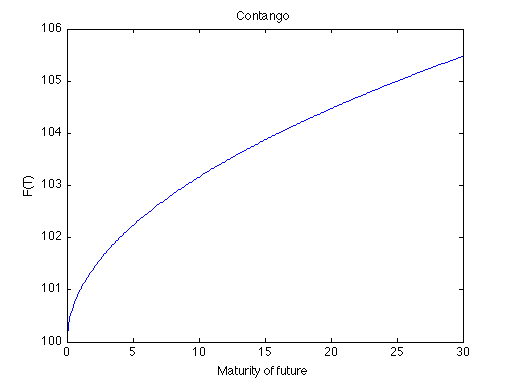
\includegraphics[width=2in]{pics/contango.png} 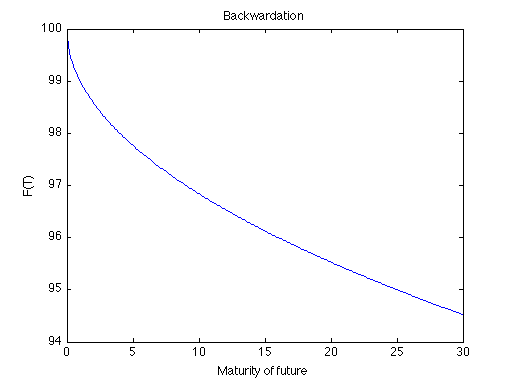
\includegraphics[width=2in]{pics/backwardation.png}   \caption{Contango and backwardation}
\label{contangoandbackwardation}
\end{center}
\end{figure}
\subsubsection{General case}

In order to hold a physical commodity for the cash and carry it is necessary to pay for storage (and possibly for any spoilage in the commodity). The storage cost can be treated much like a negative dividend. We will call the storage rate $s$.

\textit{Cash and carry:}


\begin{center} \begin{tabular}{|c|c|}
  \hline
  % after \\: \hline or \cline{col1-col2} \cline{col3-col4} ...
  time & action \\
  \hline
  t & Sell future @ $F_T(0)$  \\
    & Borrow cash $S(0)$ @ $r$ \\
    & Buy commodity @ $S(0)$ (hold in storage) \\
  \hline
 T & Deliver commodity for $F_T(0)$ \\
   & Repay loan: $S(0)(1+r)^{T} $ \\
   & Pay storage cost $F_T(0)((1-s)^{T}-1)$\\
  \hline
   & $F_T(0) - S(0)(1+r)^{T} + F_T(0)((1-s)^{T}-1)$\\
  \hline
\end{tabular}\end{center}


This transactions cannot be profitable under no arbitrage. This requires

\[F_T(0) - S(0)(1+r)^{T} + F_T(0)((1-s)^{T}-1) \leq 0 \]
\[ \Rightarrow F_T(0) = S(0)\frac{(1+r)^{T}}{(1-s)^{T}}  \]

\subsubsection{Example}

Current price: $S(t)$ = \$61\\
Borrowing/lending: $r$ = 0.05\\
Storage cost: $s$ = 0.07\\
Futures expiry: 30 days\\
Futures price upper  bound: $61((1+0.05)/(1-0.02))^{30/365}$ = \$61.35

\subsubsection{Arbitrage}

Spot crude oil sells for \$61 on June 30. A contract for delivery on July 30 delivery sells for \$64. It costs 7\% per year to store and transport the oil. The interest rate is 5\%.

\textit{Cash and carry:}

\begin{center} \begin{tabular}{|c|c|}
  \hline
  % after \\: \hline or \cline{col1-col2} \cline{col3-col4} ...
  time & action \\
  \hline
  June 30 & Sell future @ $64$  \\
    & Borrow cash $61$ @ $0.05$ \\
    & Buy commodity @ $61$ (hold in storage) \\
  \hline
 T & Deliver commodity for $64$ \\
   & Repay loan: $61(1+0.05)^1$ \\
   & Pay storage cost $64((1-0.07)^{30/365}-1)$\\
  \hline
   & $64 - 61(1+0.05)^{30/365} + 64((1-0.07)^{30/365}-1) = 2.3743$\\
  \hline
\end{tabular}\end{center}

So if the future trades at \$64 (or above) the cash and carry transaction is profitable.

\section{The operation of real world futures contracts}

Real world futures contracts have a few more complications than the examples above. The financial exposure of a contract is typically a multiple of the actual futures price. For example a NYMEX contract for oil is quoted in dollars per barrel, but the contract is actually for 1000 barrels, so if the futures price is \$70, the total value of the oil traded is \$70,000. Equity index and currency contracts are similarly multiples of the quoted price.

Exchange traded futures contracts typically use a process called \textbf{margining} to reduce credit risk. The long and short contractees each have \textbf{margin accounts} containing a fraction of the total value of the contracts (typically around 10\%). Margin accounts are are used to finance short term moves in the value of the contracts. If a margin account balance gets too low a \textbf{margin call} occurs: the account must be topped up or the position closed with an offsetting trade. Because margining occurs daily, and the margin accounts are large enough to finance a large move in the underlying price, there is greatly reduced risk that someone who enters into a futures contract will default on their obligations. 

Margining also allows for substantial \textbf{leverage} since only a fraction of the total exposure is required in the margin account to sustain a position. 

Consider an example: Say we hold 50 futures contracts on a security priced in domestic currency. The contract size is \$1000 $\times$ the underlying security price. Let's see what happens when the contract price moves from 100 to 105 if the margin is 10\% of total contract value.

\begin{center} \begin{tabular}{|c|c|c|}
  \hline
  % after \\: \hline or \cline{col1-col2} \cline{col3-col4} ...
  Today& price & 100 \\
  & contract value & \$100,000 \\
  & value of portfolio & \$5,000,000 \\
  & margin & \$500,000 \\
   \hline
  Tomorrow & price & 105 \\
  & contract value & \$105,000 \\
  & value of portfolio & \$5,250,000 \\
  & margin & \$525,000 \\
  \hline
\end{tabular}\end{center}

The position has a profit of \$5,250,000-\$5,000,000 = \$250,000. The margin increases by \$25,000. The long position receives \$225,000 (250,000-25,000) in additional cash and has a profit of \$250,000. A \$250,000 return on an initial margin of \$500,000 for a 5\% move represents a lot of leverage. However typically a portfolio funding a futures position will have substantially more than the margin. If the concept of leverage is sensible (and it often isn't) it's more natural to measure the return against the portfolio capital. In the previous example the portfolio might be \$10,000,000 (return would be 2.5\%) or \$1,000,000 (return would be 25\%).

\section{Margining and why currency risk doesn't matter much}

Futures contracts are denominated in currency, usually US dollars. It seems logical that the futures carry a full exposure to currency moves: logical but wrong. Provided that the profit or loss is margined regularly the currency exposure is very limited. We can see this by considering the effect of a currency move on the cashflows from a futures contract. To make things simple we'll consider a futures contract on a non-dividend paying equity. In the example we have an US dollar denominated futures contract and an Australian dollar denominated bank account.

Say initially the currencies are at parity (USD1 = AUD1) and the futures price is USD100. Overnight the Australian dollar devalues to USD0.9. The value of a portfolio containing one futures contract is affected as follows.


\begin{center} \begin{tabular}{|c|c|c|}
  \hline
  % after \\: \hline or \cline{col1-col2} \cline{col3-col4} ...
  Today& price & USD100 \\
  & contract value & USD100,000 \\
  & value of portfolio & USD100,000 (AUD100,000) \\
  & margin & USD10,000 (AUD10,000) \\
   \hline
  Tomorrow & price & USD100 \\
  & contract value & USD100,000 (AUD90,000) \\
  & value of portfolio &USD100,000(AUD90,000)  \\
  & margin & USD10,000 (AUD9,000) \\
  \hline
\end{tabular}\end{center}

Our margin account denominated in USD has decreased in value by AUD1000 which is quite small considering the size of the currency move. This is because currency changes only affect the margin which is typically only a portion of the total portfolio value.


\section{Questions}

\textbf{Question 1:}\\

Consider a non-dividend paying stock in the following situation:

\begin{center}
\begin{tabular}{|c|}
\hline
Current price: $S(t)$ = \$14.5\\
Borrowing/lending: $r$ = 0.1\\
Futures expiry: 1 year\\
Futures price: \$14.5\\
\hline
\end{tabular}
\end{center}

\textbf{(a)} Construct an arbitrage to take advantage of the mispricing. How much money can you make?\\
\textbf{(b)} Redo part (a) assuming the repo rate is 2\% per year.

\medskip

\textbf{Question 2:}\\

Consider the following situation in the foreign exchange market:

\begin{center}
\begin{tabular}{|c|}
\hline
Exchange rate (domestic for foreign): 0.67\\
Domestic interest rate: 0.15\\
Foreign interest rate: 0.01\\
Future exchange rate (domestic for foreign): 0.68\\
\hline
\end{tabular}
\end{center}

\textbf{(a)} Construct an arbitrage to take advantage of the mispricing. 

\medskip

\textbf{Question 3:}\\

Consider the following situation in the market for gold:

Spot gold sells for \$900 on June 30. A contract for delivery on August 30 delivery sells for \$920. It costs 1\% per year to store. The interest rate is 5\%.

\textbf{(a)} Construct an arbitrage to take advantage of the mispricing. \\
\textbf{(b)} Suppose instead that the forward price was \$900.1 and it is possible to repo gold for 0.5\% per year. Construct the arbitrage.

\medskip

\textbf{Question 4:}\\


\textbf{(a)} Consider the futures contract in the picture. If you currently hold 100 of these contracts on 10\% margin and the futures price moves to \$70 overnight what are your cashflows in USD?\\
\textbf{(b)} What are your cashflows in AUD assuming that the exchange rate is constant at 0.7.\\
\textbf{(c)} What are your cashflows in AUD assuming that the exchange rate moves from 0.7 to 0.62.

\begin{center}
  % Requires \usepackage{graphicx}
  \includegraphics[width=5in]{pics/cln9des} \\
  \textit{Futures contract on crude oil}
\end{center}


\chapter{Options pricing}


\section{The basics}

An option gives the right to buy seething at a pre-agreed price at some time in the future. For example there might be an option to buy a tonne of wheat next month for \$100. The option has value because the pre-agreed price may be lower than the market price next month. It may also have no value if the pre-agreed price is higher. 

On the outside options a slightly boring but useful workhorse financial contract. But there are some surprises under the surface. The first surprise is in the pricing. It seems logical that the price of an option should be the expected (average) value of the contract. Logical but wrong. The arbitrage-free price of an option is a function of the \textbf{volatility} of the underlying price. That discovery and it's specifics was impressive enough to warrant a Nobel Prize it's inventors: Fisher Black, Myron Scholes, and Robert Merton. 

A related and even more surprising property of option prices is that they contain a market prediction of the \textbf{probability distribution} of the price in the future. So for example it is possible to know the precise probability assigned by the market to the price of corn being above \$100 next week, or the fed funds rate being below 2\% in one year's time. These market implied probabilities are called \textbf{risk neutral probabilities}. They are very important and useful. 

We start with risk neutral probabilities in a more natural environment of simple bets and move to show how they relate to option prices. 

Unless you have a very strong mathematical background you're unlikely to fully understand the derivation of the Black-Scholes-Merton pricing formula. We won't dwell on it and if it seems strange and unnatural to you that's normal. But if you follow the logic of the simple example you'll understand broadly how it worlds, if not the fine detail.

\section{Notation}


\begin{itemize}
\item A call option with strike $K$ and expiry $T$ is dented $C_{K,T}$
\item A risk free bond paying $1$ at time $T$ is denoted $Z_T$
\item The value of any contract $x$ at time $t$ is denoted $V_x(t)$. So $V_{C_{K,T}}(t)$ is the value at time $t$ of the call option with strike $K$ and expiry $T$
\item The probability of an event is denoted $P(.)$. So $P(A)$ is the probability of an $A$ occurring. 
\end{itemize}

\subsection{Introduction to risk neutral probabilities}
A bit of motivation: The simplest kind of bet is on a single outcome (let's call it $A$) that may or may not occur. If $A$ occurs the bet pays  \$a, otherwise you get nothing. Bets on horse races and poker games are of this kind.

In such bets it is easy to establish the implied probability of $A$ occurring. It's the probability that makes the expected value of the bet equal to zero. 

\begin{eqnarray*}
\underbrace{P(A)}_{\mbox{probability}}\underbrace{1}_{\mbox{payoff}} + \underbrace{(1-P(A))}_{\mbox{probability}}\underbrace{0}_{\mbox{payoff}} = a \\
\Rightarrow P(A) = a
\end{eqnarray*}

We multiplied the probability of $A$ occurring by the \$1 prize and added the probability of $A$ not occurring $(1-P(A))$ by the \$0 prize. A more general bet pays $Z_1$ if $A$ happens and $Z_2$ if it doesn't:

\begin{eqnarray*}
P(A)Z_1 + (1-P(A))Z_2 = a \\
\Rightarrow P(A) = \frac{a-Z_2}{Z_1-Z_2}
\end{eqnarray*}

In either case the probability implied by the price of the bet is derived by setting the price equal to its \textbf{expected value}. If these were the true probabilities then a \textbf{risk neutral} investor would be indifferent between taking the bet or not. That's why they're called \textbf{risk neutral probabilities}. Under certain circumstances the risk neutral probabilities will be associated with prices which are \textbf{arbitrage free} in the sense that we can't trade these prices and make money with no risk. 

What does any of this have to do with options? It turns out that you can extract risk neutral probabilities from option prices in a similar way to extracting them from a simple bet on an event. This is a very useful way to think about  (and price) options.

\subsection{What's an option?}

An \textbf{option} is a contract that gives its owner the option to buy or sell something for a fixed price at a later date. For example I might buy an option to buy a can of beans for \$2 in two months time. If the prevailing price for a can of beans after two months is higher than \$2, the option has value, if it's lower the option is worthless (there's no point in buying the beans for \$2 when they only cost \$1.50.)

If the price of beans turns out to be \$3 after two months the option is worth \$1 because you save \$1. If the price is \$10 the option is worth \$8. The final value of the option as a function of the future price of beans looks like this:

\begin{center}
  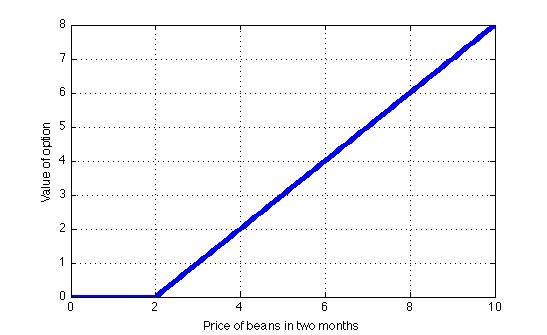
\includegraphics[width=3in]{pics/beanscall.png} 
\end{center}

This type of contract is called a \textbf{call option}. A call option has a \textbf{strike price} (\$2 in example above) and an \textbf{expiry} (two months time). There are also \textbf{put options} which give the option to sell at a certain price. A put option on beans with a strike price of \$2 and a 2 month expiration would look like this:

\begin{center}
  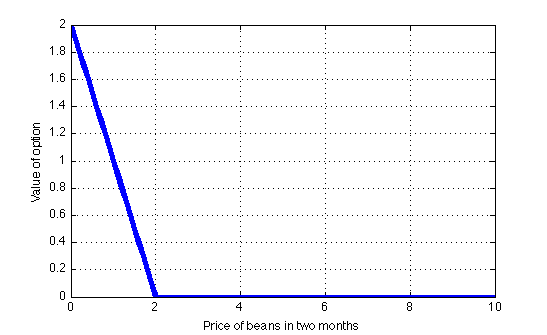
\includegraphics[width=3in]{pics/beansput.png} 
\end{center}


\section{Extracting risk-neutral probabilities from option prices}

Figure \ref{call} is the payoff of a call option to buy something denoted $S$ at a future time $T$:

 \begin{center}
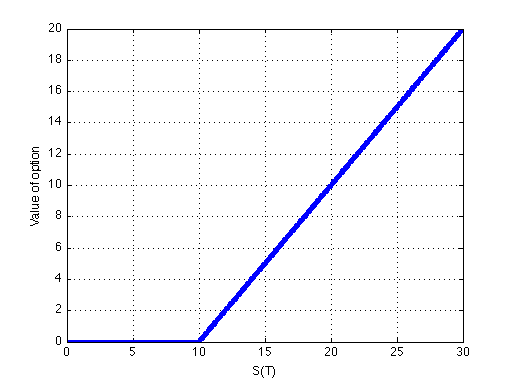
\includegraphics[width=3in]{pics/calloption}%
\captionof{figure}{A call option}\label{call}%
\end{center}

Figure \ref{simple} is the payoff of a simple bet

 \begin{center}
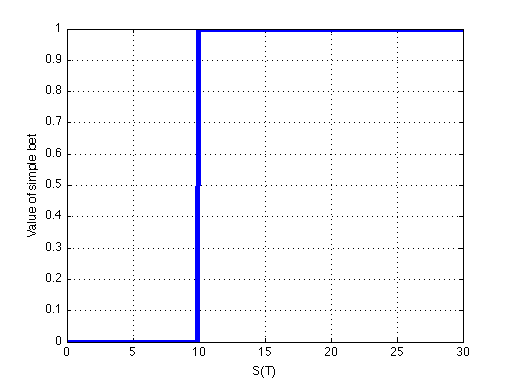
\includegraphics[width=3in]{pics/simplebet}%
\captionof{figure}{A simple bet}\label{simple}%
\end{center}


To construct a simple bet from call options, buy a call option at strike $K$ and sell a call option at  a nearby strike $K+\delta$. The combined portfolio is worth 0 if the price at expiry is less than $K$, $\delta$ if the price is greater than $K+\delta$, otherwise $S(T)-K$.

The value of the security underlying the option will be called $S(t)$. The option expires at time $T>t$. 

\begin{eqnarray*}
\mbox{Bought call at strike $K$ + Sold call at strike $K+\delta$ }&= +C_{K,T}-C_{k+\delta,T}\\
&= 
\begin{cases} 
0 \mbox{ if } & S(T)\leq K \\ 
S(T)-K \mbox{ if} &K < S(T)< S(T)+\delta \\
 \delta \mbox{ if } &S(T)  \geq K+\delta 
 \end{cases} 
 \end{eqnarray*}

The first panel in figure \ref{callToSimple} is the bought call at strike $K$, the second panel is the sold call at strike $K+\delta$. The third panel is the combined payoff. (In this example the first strike is 10 and the second strike is 11 so $\delta = 1$.)
 
 \begin{center}
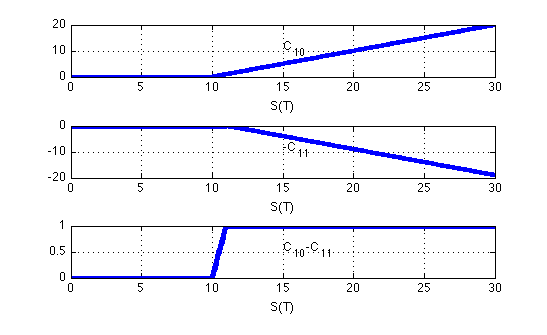
\includegraphics[width=4in]{pics/callspread}%
\captionof{figure}{Constructing a simple bet from call options}\label{callToSimple}%
\end{center}
 

Provided that $\delta$ is small this portfolio is very similar to a simple bet. As $\delta$ approaches 0, it approaches a bet that pays 0 if the price at expiry is less than $K$ and $\delta$  if the price is greater than $K$. If the price of an option at $K$ is $V_{C_{K,T}}$ then the total portfolio costs $V_{C_{K,T}}-V_{C_{K+\delta,T}}$.

Recall in the introduction we established that a bet that pays $Z$ if an event happens and $0$ if it doesn't and costs $a$ implies a probability of $A$

\[P(A) = \frac{a}{Z}\]

In our current example the 'event' $A$ is the price being greater than $K$, and the probability is

\[P(A) = \lim_{\delta \rightarrow 0} \frac{V_{C_{K,T}}-V_{C_{K+\delta,T}}}{\delta} \]

If $C$ is a differentiable function (let's say it is) this is actually just the first derivative of the function $V_{C_{x,T}}$ evaluated at $x=K$

\[ P(A) = \frac{\partial V_{C_{K,T}}}{\partial K} \]

More precisely

\[ P(S(T) \geq K) = \frac{\partial V_{C_{K,T}}}{\partial K}\]

This is a really nice result. It means that if we have option prices for a security at some expiry we have a (risk neutral) probability distribution for the price. If someone asks ``what's the probability that the USD/JPY exchange rate will be above 150 by next year?'' we can give a probability consistent with market prices. It also means that anybody who disagrees with the risk neutral distribution can place a trade against it. This leads to a much richer set of trading strategies than just punting if something will go up or down.

%It's also a good example of the fundamental theorem of arbitrage free prices which says that arbitrage free prices are associated with a unique risk neutral probability distribution. 

\section{How do we get $V_{C_{K,T}(t)}$?}
If we have some function that gives us option prices then we have the risk neutral probability distribution and all is well. But how do we get it? There are two common approaches to explaining option pricing -- both are fairly unintelligible if you don't have a mathematical background. However the basic idea is quite simple. If you can grasp the one big idea it's not so important if you follow the minutiae.


\subsection{The big idea}

We've already seen that there is a relationship between the arbitrage free price and a risk neutral probability. But we don't yet know how to get the correct price. The big idea behind arbitrage free pricing is that the price of an option should be such that we cannot create an arbitrage. We can figure out what the correct price (and probability) is by assuming there is no arbitrage and working backwards.

This is an important idea because it divorces the price of a security from how much a subjective investor might expect it to be worth on average, or how risky it is, or any other consideration. Everything comes down to arbitrage.

The price of the option at time $t$ is given by the value function $V_{C}(t)$. That's what we're making.

%Doing so requires an arbitrage free framework to hedge the instrument: our goal is the price of the hedge is the price of the security. There will be some risk neutral probabilities associated with the correct prices, and we know how to make those from the last section.

%Unfortunately there is no really simple way to describe how these prices and probabilities are obtained. There are intuitive explanations, but they leave a lot of questions. There is an approach which perfectly describes the core process driving the hedge, while actually describing a different kind of hedge. That's a good starting point. It gives the tools to understand the process at play. And stopping there is fine. So is extending the framework to describe the exact type of arbitrage relationship that defines option prices and their associated probabilities.

\subsection{One period, two states}

We'll consider a very simple market with only two possible outcomes. The arbitrage logic in this scenario is the same as in more complicated scenarios. 

\subsubsection{Pricing options by arbitrage}
Suppose we are in a market with an asset priced at $S$. The asset has two possible future states: \textit{up} or \textit{down}. In the up state it's worth $S_u = S(1+u)$, $u>0$; in the down state it's worth $S_d = S(1+d)$, $d<0$ Call options are available for this market. In the 'up' state the call is worth $V_{C_u} = \max(S_u-K,0)$. In the 'down' state it's worth $V_{C_d} = \max(S_d-K,0)$ In this market you can borrow or lend at a rate $r$. We'll impose that $d<r<u$.

Now we construct a portfolio with $h$ shares of the stock and -1 call (so we sell the call). This portfolio will have two possible values depending which state occurs

\begin{eqnarray*}
V_u = hS_u -V_{C_u}\\
V_d = hS_d -V_{C_d}
\end{eqnarray*}

Our strategy will be to make this portfolio worth the same amount in either case. If we achieve that the portfolio will be \textbf{riskless}. A riskless portfolio will only return the risk-free rate $r$, otherwise there would be an arbitrage (we could borrow/lend at $r$ and buy/sell the riskless portfolio).

This is easy:

\begin{eqnarray*}
hS_u -V_{C_u} = V_u = V_d = hS_d - V_{C_d}\\
\rightarrow h = \frac{V_{C_u}-V_{C_d}}{S_u-S_d}
\end{eqnarray*}
 
The portfolio costs $hS-C$. For no-arbitrage to hold the discounted value of both $V_u$ and $V_d$ (they're the same now) must be equal to $hS-V_{C}$. This gives us enough information to solve for $V_{C}$

\begin{eqnarray*}
\frac{hS_u-C_u}{1+r}= hS-V_{C}\\
\rightarrow V_C = \frac{p V_{C_u}  + (1-p) V_{C_d}}{1+r}
\end{eqnarray*}

Where $p = \frac{r-d}{u-d}$. There's a bit of rearranging needed to get this but it's all straightforward (check it yourself). In this form it's also clear that the risk-neutral probability of the 'up' state is $p$. If we substitute back for $p$, $V_{C_u}$ and $V_{C_d}$ we get

\[V_{C} =\frac{r-d}{u-d} (S(1+u)-K)(1+r)^{-1}\]

We could have found the risk neutral probability first and then priced the option. We'll do that in the next section.
 
\textbf{Example:}\\

We'll set up an incorrect call price to create the arbitrage and then solve for the correct price. We face the following two state market:

\begin{itemize}
\item Current price:  $S = 100$
\item Interest rate: $r = 0.25$
\item Up move: u = 2 ($S_u =  S(1+u) = 30$)
\item Down move: d = -0.5 ($S_d = S(1+d) = 5$)
\item Call option strike: $K =10$ 
\item Call price: $V_C = 5$
\end{itemize}


Recall the arbitrage portfolio is short 1 call option and long $h$ units of the stock where $h$ is

\[ h = \frac{V_{C_u} - V_{C_d}}{S_u-S_d} = \frac{20 - 0}{30-5} = 0.8\]

If the \textit{up} state occurs we get $hS_u-V_{C_u} = .8*30-20 = 4$. If the \textit{down} state occurs we get  $hS_d-V_{C_d} = .8*5-0 = 4$. The portfolio costs $hS -V_{C} = .8*10-5 = 3$. If we borrow \$3 now and invest in the portfolio we have to pay back \$3.75. We get an \textbf{arbitrage profit} of .25 no matter what happens.

\begin{center} \begin{tabular}{|c|c|c|}
  \hline
  % after \\: \hline or \cline{col1-col2} \cline{col3-col4} ...
  & \textit{up} & \textit{down}\\
  \hline
  now & borrow \$3 & borrow \$3 \\
           &buy 0.8 units of $S$ &buy 0.8 units of $S$\\
           &sell 1 call & sell 1 call\\
  \hline
  1 year & repay 3*(1+.25) = 3.75 & repay 3*(1+.25) = 3.75\\
              & sell 0.8*30 = 24 & sell 0.8*5 = 4\\
              & pay call (30-10) = 20 & pay call 0\\
  \hline
             & 24-20-3.75 = 0.25 (arbitrage profit) & 4-0-3.75 = 0.25 (arbitrage profit)\\
             \hline
\end{tabular}
\end{center}

The risk-neutral probability is 
\begin{eqnarray*}
p = \frac{r-d}{u-d} =0.3
\end{eqnarray*}

The arbitrage free price is

\begin{eqnarray*}
C = \frac{p V_{C_u}  + (1-p) V_{C_d}}{1+r}\\
 = p(S(1+u)-K)(1+r)^{-1} \\
= 0.3(30-10)(1+0.25)^{-1} = 4.8
\end{eqnarray*}


\subsubsection{The easy way}

We already have the arbitrage free price and the risk neutral probability, but it's interesting and instructive to get it in another way. 

The price $S$ is the discounted expectation of the two states using risk-neutral probabilities. Call the probability of the \textit{up} state $p_u$ and the \textit{down} state $p_d$
 
 \[S = (p_u S_u + p_d S_d)(1+r)^{-1}\]

The price is the discounted expectation under the \textbf{risk neutral} probabilities. Since $p_d = (1-p_u)$, and substituting for $S_u$ and $S_d$ we have

\[S = (p_u S(1+u) + (1-p_u)S(1+d))(1+r)^{-1}  \]

Solving for $p_u$ gives

\[ p_u = \frac{r-d}{u-d}\]
and
\[p_d = \frac{u-r}{u-d} \]

With these risk-neutral probabilities we may price the option. The discounted expected value of a call option with strike $K$ is

\[V_C = (p_u V_{C_u}+ p_d V_{C_d})(1+r)^{-1}\]

Substitute in $C_u = S(1+u)-K$ and $C_d = 0$

\[C = \frac{r-d}{u-d} (S(1+u)-K)(1+r)^{-1}\]

This is the arbitrage free price for the call option in this two-state model. 

Markets with more periods and more states are priced in the same way. First we determine a set of probabilities (or probability distribution) which make the price equal to its discounted expectation \textit{at each point in time}. Then we use those probabilities to price the value of the option by taking the discounted expectation of the value of the call in each scenario.


\section{The real formula}

Real world markets do not have two states and one period. The correct price of an option is generated by a similar process as the two-state model, by ensuring that the probabilities are \textbf{risk neutral} and the price \textbf{arbitrage free} for \textit{every possible state at every possible time}. 

This is not the place to derive these more complicated models. We will simply state without proof that the correct price of a call option for \textbf{continuous time} ($T$ periods, infinitely divisible) with an \textbf{infinite number of possible states} (S can go from 0 to infinity) is

\begin{eqnarray}
V_{C(K,T)}(t) = N(d_1)S - N(d_2)Ke^{-r(T-t)}\\
d_1 = \frac{\ln \frac{S}{K} + r+\frac{\sigma^2}{2}(T-t)}{\sigma \sqrt{T-t}}
d_2 = \frac{\ln \frac{S}{K} + r-\frac{\sigma^2}{2}(T-t)}{\sigma \sqrt{T-t}}
\end{eqnarray}

Where $\sigma$ is the standard deviation of the underlying asset returns\footnote{A return is $r=\log(S(t+1)/S(t))$. This is a random variable and has a standard deviation $\sigma = $}, $t$ is the current time, and $N(.)$ is the cumulative distribution function of the standard normal distribution.\footnote{Which is $\int_{-\infty}^x \frac{1}{2\pi}e^{-\frac{x^2}{2}}dx$}
 
The derivation is a extension of the single-period two-state model, but it uses the central limit theorem and something called It$\hat{o}$ Calculus. 

%If you don't understand the central limit theorem you really should be doing that before worrying about option prices. You should also be worrying about the decisions you've made in life.

\textbf{An incorrect objection}

One objection is that price changes don't follow a normal (Gaussian) distribution, and the formula has the form of a Gaussian distribution in its pricing function. People who make this criticism and don't understand the logic of Black-Merton-Scholes. The central limit theorem says that a sufficiently large number of draws from \textit{any} distribution, no matter how peculiar, will be normally distributed. Black-Merton-Scholes uses this in the derivation. The distribution of price movements doesn't matter provided that it doesn't change. If it does change, the sums aren't from an identical distribution, and so you have to deduce the arbitrage free price in a more complicated way. But if the distribution is constant, then no matter how peculiar, or skewed, or `fat-tailed' the distribution is, Black-Merton-Scholes holds.

%There's another kind of incorrect objection: that options are a \textbf{redundant security}. This claim derives from the fact that in a Black-Merton-Scholes world, you can replicate an option price exactly with an appropriate trading strategy on the underlying security, Therefore in that world there is no need to buy options, you can just make them yourself. That makes them redundant: you could live without them.  

%But in the real world nobody ever knows what the volatility is. An option is implicitly a bet that the volatility of the underlying security will be $\sigma$. There's no other way to bet on volatility. Even if the price dynamics go completely off the rails there's going to be a risk neutral probability distribution. It allows us to answer questions like ``what's the probability that the Google Inc. will trade above 500 in a year's time?" We can't answer that question in an arbitrage free way without options. 

And that's it. That's option pricing. 

\section{What about $P_K$?}

All of this has been about call options. The same arbitrage logic can be used to price put options, but you don't need to worry about the details because the price of call and put options is connected by an arbitrage relationship called \textbf{put-call parity}

\subsection{Put-call parity}

Say we have call and put options both at strike $K$ (first and second panel of figure \ref{comboToFuture}). A portfolio of a call option and a sold put (panel 3) gives us a straight line (panel 4). 

Now if we add a sold future with the same expiry (first panel of figure \ref{comboToArb}) as the call and put (panel 2) we get an unchanging payoff (panel 3). If this line is above zero we have an arbitrage. It follows that if we know the call price and the futures price we can figure out an arbitrage free put price. The details are below

 \begin{center}
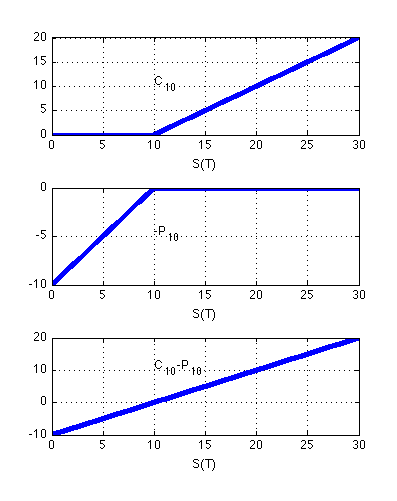
\includegraphics[width=4in]{pics/cpf}%
\captionof{figure}{A bought call plus a sold put is like a future}\label{comboToFuture}%
\end{center}


 \begin{center}
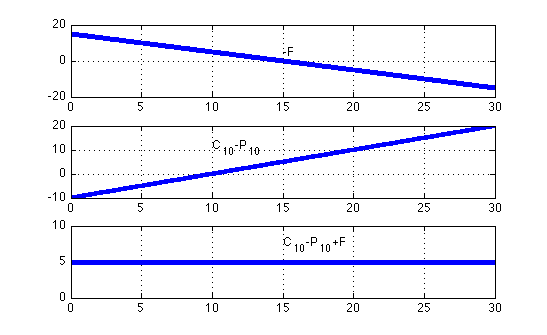
\includegraphics[width=4in]{pics/cpfarb}%
\captionof{figure}{A bought call plus a sold put plus a sold future is an arbitrage}\label{comboToArb}%
\end{center}


\begin{center}
\begin{tabular}{|l|c|}
\hline
now &Borrow/Lend $V_{C_K} - V_{P_K}$\\
	&Buy 1 call for $V_{C_K}$\\
	&Sell 1 put for $V_{P_K}$\\
	&Sell 1 future for F\\
\hline
one year
	       & repay/receive ($V_{C_K}-V_{P_K})(1+r)$\\ 
	       & Receive $(S-K)^+$\\
	       & pay $(K-S)^+$ on the put\\
	       & deliver futures contract for F-S\\
	       \hline
	       &$S-K + (F-S) - (V_{C_K}-V_{P_K})(1+r) = F-K - (V_{C_K}-V_{P_K})(1+r)$\\
	       \hline
\end{tabular}
\end{center}

The no-arbitrage condition is

\begin{eqnarray*}
F-K - (V_{C_K}-V_{P_K})(1+r) \leq 0\\
V_{C_K} - \frac{F-K}{1+r} \geq V_{P_K}
\end{eqnarray*}

The arbitrage works in reverse too (sell the call, buy the put, buy the future) and produces

\[ V_{C_K} - \frac{F-K}{1+r} \leq V_{P_K}\] 

Since it must be both greater than or equal to \textit{and} less than or equal to, it must be equal to

\[ V_{C_K}- \frac{F-K}{1+r} =  V_{P_K}\] 

\section{Questions}

\textbf{Question 1:}\\
An online betting company is offering \$5 for Pakistan to win against India in the cricket. What's the risk-neutral probability of Pakistan winning?

\textbf{Question 2:}\\
A bookie is offering 5:2 odds on for the horse 'Mr Pinkerton" in the third race. What is the risk neutral probability of Mr Pinkerton winning the race?

\textbf{Question 3:}\\
Suppose the price of a call option is given by the function $V_{C_K} = \ln(K)$. What is the probability that the price will be above \$5 at expiry? 


\textbf{Question 4:}\\Suppose the price moves only in increments of \$1. Use the options from question 3 to construct a simple bet that the price will be above \$10 at expiry. What is the arbitrage free price of this bet? What is the risk-neutral probability?


\textbf{Question 5:}\\The following situation prevails in a two-state market
\begin{itemize}
\item Current price:  $S = 10$
\item Up move: u = 6 ($S_u =  S(1+u) = 70$)
\item Down move: d = -1 ($S_d = S(1+d) = 0$)
\item Interest rate: r = 0.25
\item Call option strike: $K =10$ 
\item Call price: $V_C = 5$
\end{itemize}

 \begin{enumerate}
 \item Construct an arbitrage to take advantage of the mispriced call.\\
\item What are the risk-neutral probabilities of the \textit{up} and \textit{down} states.
\end{enumerate}

\textbf{Question 6:}\\A call at a strike of 10 costs \$5. The futures contract trades at $10$. What is the correct price of the put if the interest rate is 25\%?

\textbf{Question 7:}\\
Construct an arbitrage if the put costs \$6


%Consider two investment strategies

%Strategy 1:
%\begin{itemize}
%Start with \$B in cash
%Borrow a further \$R and invest the \$(R+B) in the stock (R = B\frac{1}{\frac{1+r}{1+d}-1})
%\end{itemize}

%Strategy 2:
%Buy $X$ options on the stock ($X = \frac{(B+R)(1+u)-R(1+r)}{Su}$)

%The payoff of strategy in both states is in the table below

%Strat1,u (R+B)(1+u)-(1+r)R
%Strat1,d (R+B)(1+d)-(1+r)R = 0

%Strat2,u X (S(1+u)-S) = XSu = \frac{(B+R)(1+u) - (1+r)R }{Su}Su = (B+R)(1+u) - (1+r)R
%Strat2,d  0 

%Strategy 1 and 2 pay the same amount in either state, they are perfect substitutes so they must have the same price or there will be an arbitrage. Strategy 1 costs \$B, strategy 2 costs \$XC. So it must be that C = B/X. This is the arbitrage free price of the call option.

%Substituting for $X$ gives 

%\begin{eqnarray}
%C = SuB/[(B+R)(1+u) - (1+r)R]
 % =  Su/[(1+R/B)(1+u) - (1+r)R/B]
 % = Su/[(1+\frac{1}{\frac{1+r}{1+d}-1})(1+u) - (1+r)\frac{1}{\frac{1+r}{1+d}-1}]
%\end{eqnarray}

%So the value of the call option is a function of $S$ $u$, $d$, and $r$.

%The risk neutral probability can be making the expected value of a call option equal to zero. If we get the 'up' state we get Su-C and if we get the 'down' state we get -C. So:

%\begin{eqnarray}
%P(u)(Su-C)  + (1-P(u))*-C = 0\\
%\rightarrow P(u) = \frac{Su}{C} =  \frac{(B+R)(1+u)-R(1+r)}{B} = (1+R/B)(1+u)-R/B(1+r)
%\end{eqnarray}

%Substituting for $R$ gives

%\begin{eqnarray}
%P(u) = (1+\frac{1}{\frac{1+r}{1+d}-1})(1+u)-\frac{1}{\frac{1+r}{1+d}-1}(1+r)
%[reduced form]
%\end{eqnarray}

%This is also a simple bet that we know about. It provides a risk-neutral probability and an arbitrage free price with a very simple technique. It has similar qualities as a 'heads or tails' game.

%Here's you:

%(picture)

%and here's your decisions with their possible consequences and probabilities.

%(picture)

%If it goes 'up' the call option gives you a dollar, and you have to pay for the option which is priced \$C, so you get 1-C(1). If the option goes down the option pays nothing but you still have to pay for it so you get $-C(1)$. You can borrow or lend any amount of money at rate $r$.

%In this world you can do a combination trade. If it costs the same to produce two trades and the trades have a different price you have a potential arbitrage, and that's not allowed.
 
%You face the following investment opportunities:

%Strategy 1:


%[example]

%The prices are different if the price of the option is less than or equal to X. The same logic holds if you do the opposite, so it has to be greater than or equal than X. We can deduce that the price must be exactly X. Then we have arbitrage free prices and risk neutral probabilities, we're set. 

%Now you might ask what about if there are another set of prices that are also arbitrage free. What then? That's a stupid question. Intuitively the price and probability must be unique. Otherwise there would be a trivial arbitrage buying one set of prices and selling another. And in that case they wouldn't be arbitrage free. Would they?

%That's it. That's the two-state one-period binomial problem.


%\subsection{}

%What we might want to do is expand this definition by looking at a n-state n-period binomial problem. It looks like this:




\newpage
\pagestyle{plain}
\addcontentsline{toc}{chapter}{Bibliography}
\bibliographystyle{elsart-harv-ms}
\bibliography{finalreportrefs}
\newpage

\end{document}
